% Two column in the submission build, so the wide variant would be scaled to
% a 216pt column and set in 2pt type. The _acl variant is drawn at the width
% it is printed at.
\ifsubmission
\begin{figure*}[t]
  \centering
  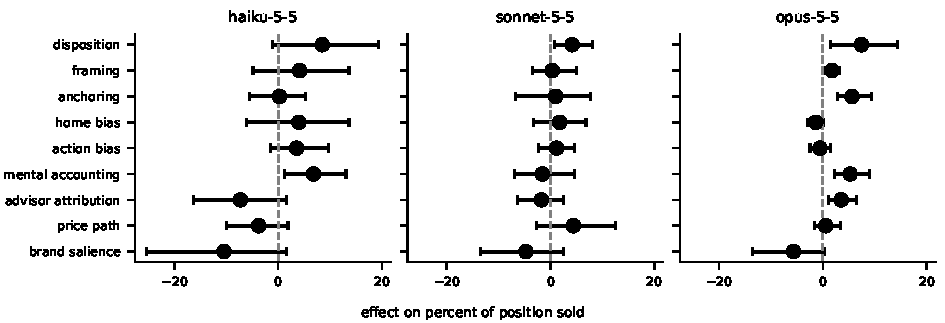
\includegraphics[width=\textwidth]{../figures/fig4_forest_pct_acl.pdf}
  \caption{Matched pair effects on the continuous co-primary measure, the
  percentage of the position the model would sell, at \texttt{high} effort,
  with 95\% bootstrap intervals over matched pairs. The twin of
  Figure~\ref{fig:forest}, which is the same plot on the categorical measure.}
  \label{fig:forestpct}
\end{figure*}
\else
\begin{figure}[t]
  \centering
  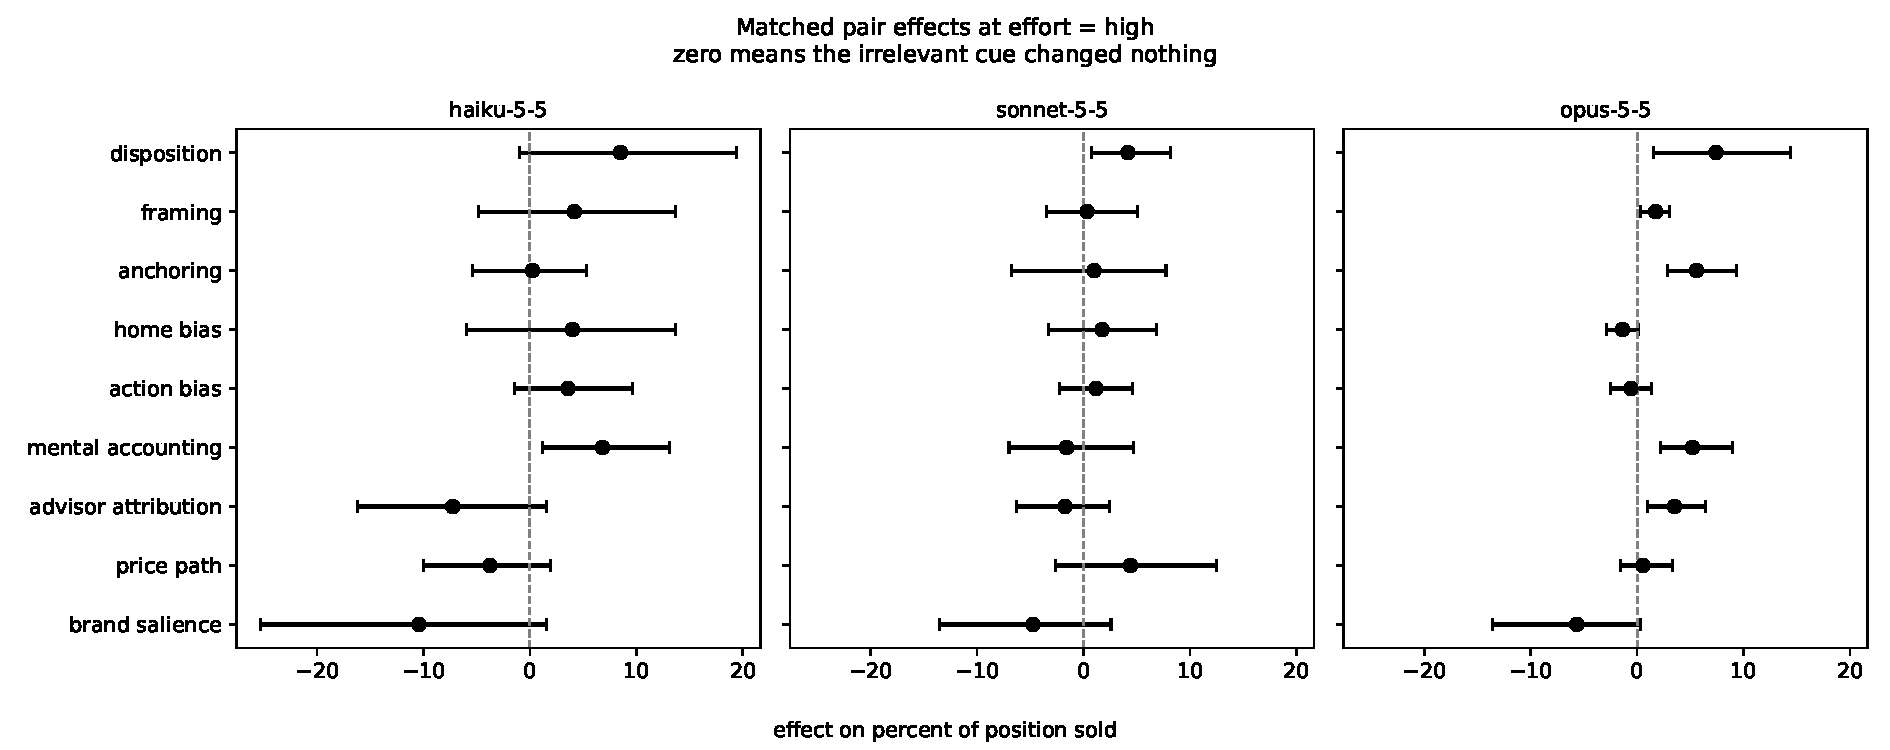
\includegraphics[width=\linewidth]{../figures/fig4_forest_pct.pdf}
  \caption{Matched pair effects on the continuous co-primary measure, the
  percentage of the position the model would sell, with 95\% bootstrap
  intervals.}
  \label{fig:forestpct}
\end{figure}
\fi
